\chapter{The AL Language}
\label{sec:appendix-allang}

One of the main design aspects of \emph{Business Central} (BC) is that all business logic is written in 
a custom Application Language (AL), hiding all implementation details dealing with the technology.

Extensions can be provided for the \emph{Business Central} runtime to add business functionality
and to fit customers' requirements as much as desired. Such extensions are not only written by
Microsoft, as users can customize their experience via extensions as required.

This effectively creates an ecosystem of AL software, for diverse use cases of BC as an ERP.

Adding a language abstraction forces abstraction layers to what is possible within the language
and effectively separates business logic from technology implementation specifics.
This has allowed the product to evolve throughout the years and experience several changes 
that with a different design would be harder to achieve, for example: changing the 
database engine, or migrating to a cloud environment. Additionally, the language continues
to evolve and be actively maintained by the team, to keep up with the requirements
a modern language infrastructure requires.

Interestingly, this approach has been successfully used by other products as well. For example,
another ERP: SAP, has the language ABAP. A custom Domain Specific Language (DSL) resembling COBOL
to extend the functionality of the system.

In this section, we give a brief tour of AL, \emph{Business Central}'s custom DSL for modifying
its runtime. For a complete reference, we refer to Microsoft's documentation \cite{bcaldocs}.

\section{How does AL look?}

In terms of syntax, AL resembles Pascal. It is an imperative, and procedural language. 
As a quick overview, we show some of the basic building blocks of the language
in the following figures.

As you see, variables are \emph{typed}. The \texttt{Record} variable type corresponds to
records in a table on the underlying database of the system. As we will explain later,
a user can also define the tables to use in this language.

\begin{figure}
    \begin{minipage}{.45\textwidth}
        \begin{Verbatim}[fontsize=\tiny]
var
    myInt: Integer;
    isValid: Boolean;
        \end{Verbatim}
        \parbox{0.9\textwidth}{\caption{Variable declaration in AL.}}
        \label{fig:al-var-decl}
    \end{minipage}%
    \begin{minipage}{.45\textwidth}
        \begin{Verbatim}[fontsize=\tiny]
Amount := Total * myInt;
        \end{Verbatim}
        \caption{Assignment and operations in AL.}
    \end{minipage}
\end{figure}

\begin{figure}
    \begin{minipage}{.45\textwidth}
        \begin{Verbatim}[fontsize=\tiny]
if x = y then begin  
    x := a;  
    y := b;  
end else 
    y := b;   
        \end{Verbatim}
        \parbox{0.9\textwidth}{\caption{Branching in AL.}}
    \end{minipage}%
    \begin{minipage}{.45\textwidth}
        \begin{Verbatim}[fontsize=\tiny]
procedure MyProcedure(Arg1: Integer; 
           Arg2: Boolean): Integer
begin
    if Arg2 then
        exit(-Arg1)
    exit(Arg1)
end
        \end{Verbatim}
        \parbox{0.9\textwidth}{\caption{Declaring a procedure in AL.}}
        \label{fig:al-proc-decl}
    \end{minipage}%

\end{figure}

\section{AL objects and BC's runtime}
Objects in AL are not the general objects as understood in the Object-Oriented Programming paradigm. Instead,
they correspond to different units of BC's functionality.

Every code element in AL belongs to some object. To see the syntax of how to declare them, see figure \ref{f:appendix-alobject}.
It requires an \texttt{ObjectID} a positive integer, an \texttt{ObjectName} a string identifier, and an \texttt{ObjectType}.

\begin{figure}
    \begin{Verbatim}[fontsize=\tiny]
<ObjectType> <ObjectID> <ObjectName>
{
    // Definition of the object
}
    \end{Verbatim}
    \caption{Syntax to define an AL object.}
    \label{f:appendix-alobject}
\end{figure}

We will show some of these \texttt{ObjectType}s, and their effect on the runtime.

\subsection{The \texttt{Page} type}

Objects of \texttt{Page} type, correspond to interactive interfaces the user experience within the product.

In figure \ref{f:app-al-page-alcode} you can see the AL code used to define the page a user can interact with 
shown in figure \ref{f:app-al-page}

\begin{figure}
    \begin{Verbatim}[fontsize=\tiny]
page 379 "Bank Acc. Reconciliation"
{
    Caption = 'Bank Acc. Reconciliation';
    PageType = ListPlus;
    PromotedActionCategories = 'New,Process,Report,Bank,Matching,Posting';
    SaveValues = false;
    SourceTable = "Bank Acc. Reconciliation";
    SourceTableView = WHERE("Statement Type" = CONST("Bank Reconciliation"));

    layout
    {
        // ...
    }
}
    \end{Verbatim}
    \caption{Example of an AL page.}
    \label{f:app-al-page-alcode}
\end{figure}

\begin{figure}
    \centering
    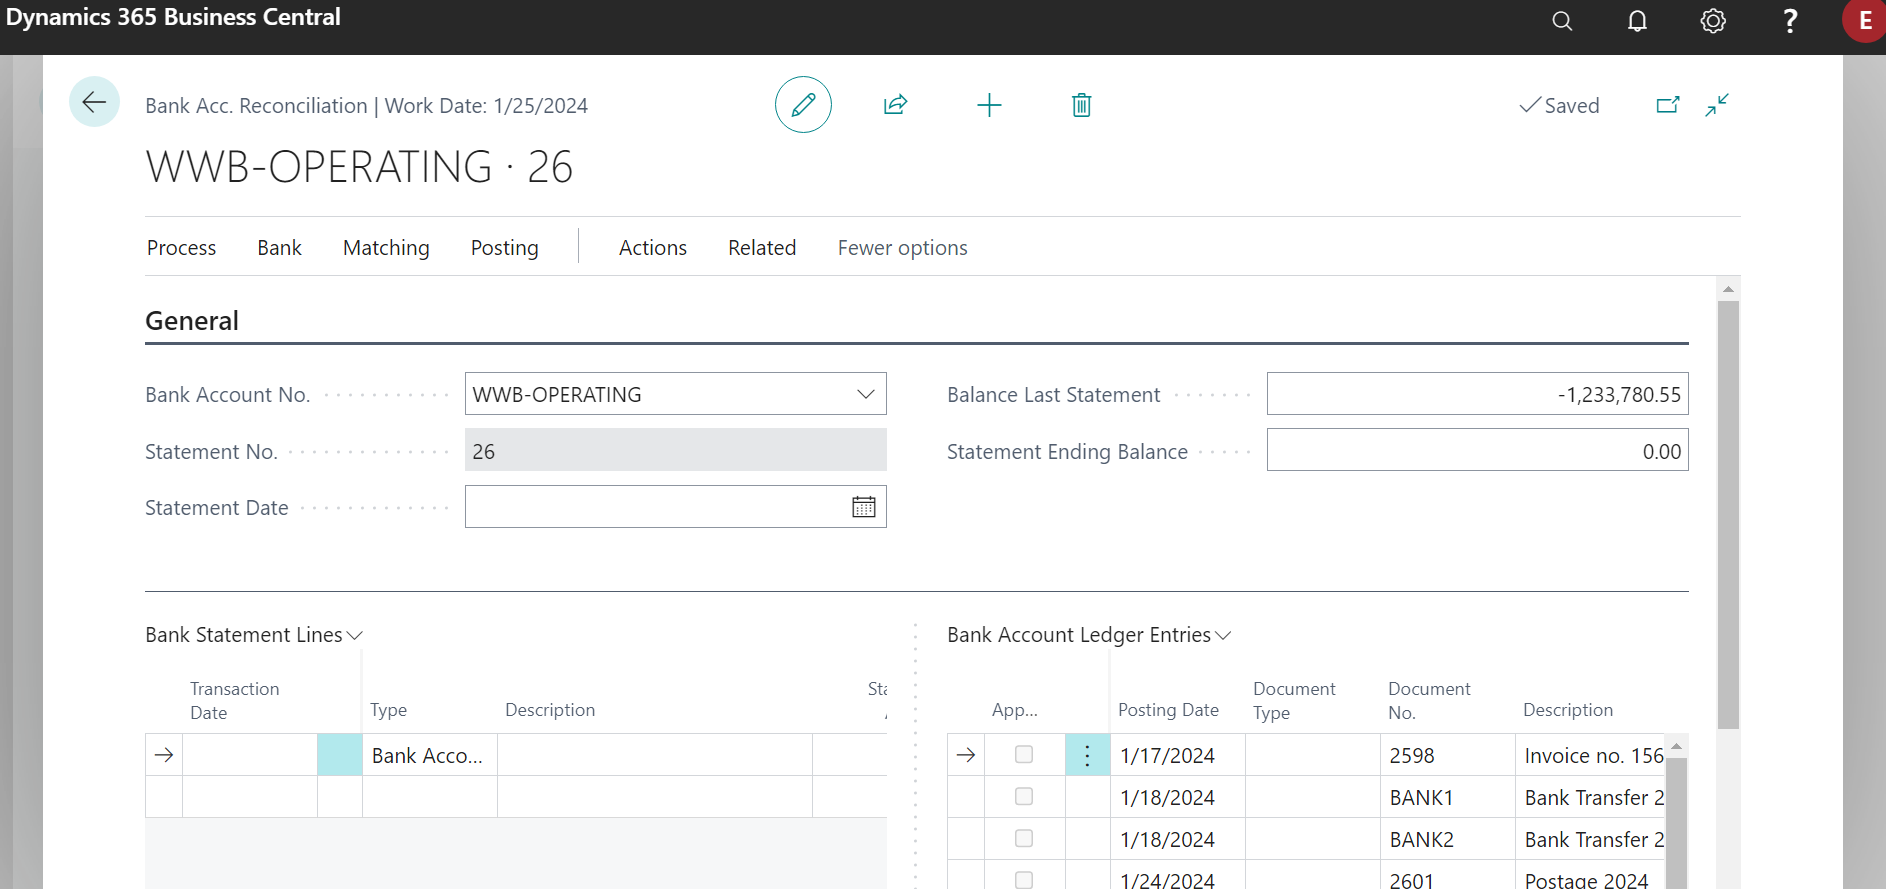
\includegraphics[width=0.9\textwidth]{thesis/figures/images/example-al-page.png}
    \caption{The interface with which the user interacts, as defined by the AL page from figure \ref{f:app-al-page-alcode}.}
    \label{f:app-al-page}
\end{figure}

\subsection{The \texttt{Table} type}

Objects of \texttt{Table} type, correspond to persistent storage in the system. Defining this object corresponds
to creating a table in the underlying SQLServer database.

Having defined a table, a developer can now use \texttt{Record} type variables of such table,
to manipulate and use this table as required, effectively acting as a data layer abstraction.

In figure \ref{f:app-al-table-alcode} you can see the definition of a table, and in figure \ref{f:app-al-record-usage}
how data can be manipulated by the usage of a \texttt{Record} variable.

\begin{figure}
    \begin{Verbatim}[fontsize=\tiny]
table 273 "Bank Acc. Reconciliation"
{
    Caption = 'Bank Acc. Reconciliation';
    DataCaptionFields = "Bank Account No.", "Statement No.";
    LookupPageID = "Bank Acc. Reconciliation List";
    Permissions = TableData "Bank Account" = rm,
                  TableData "Data Exch." = rimd;

    fields
    {
        field(1; "Bank Account No."; Code[20])
        {
            // ...
        }
        // ...
    }
    // ...
}
    \end{Verbatim}
    \caption{Example of an AL Table.}
    \label{f:app-al-table-alcode}
\end{figure}

\begin{figure}
    \begin{Verbatim}[fontsize=\tiny]
    // ...
    CurrPage.Update(false);
    if not BankAccReconciliation.IsEmpty() then begin
        BankAccReconciliation.Validate("Statement Ending Balance", 0.0);
        BankAccReconciliation.Modify();
    end;
    // ...
    \end{Verbatim}
    \caption{Example of using a record \texttt{BankAccReconciliation} of the type defined by the table in figure \ref{f:app-al-table-alcode}.}
    \label{f:app-al-record-usage}
\end{figure}

\subsection{The \texttt{Codeunit} type}

Objects of \texttt{Codeunit} type, correspond to logical units of functionality, much like \emph{modules} in 
other languages. They are a set of procedures that can be called from anywhere else within the AL codebase
with certain access modifiers.

In figure \ref{f:app-al-codeunit} you can see a procedure defined in a codeunit and in figure \ref{f:app-al-codeunit-usage}
an example of it being used from a different AL object.

\begin{figure}
    \begin{Verbatim}[fontsize=\tiny]
codeunit 18 "Financial Report Mgt."
{

    TableNo = "Financial Report";

    var
        AccSchedLine: Record "Acc. Schedule Line";
        FinRepPrefixTxt: Label 'FIN.REP.', MaxLength = 10, // ...
        TwoPosTxt: Label '%1%2', Locked = true;
    // ...
    procedure XMLExchangeExport(FinancialReport: Record "Financial Report")
    var
        ConfigPackage: Record "Config. Package";
        ConfigXMLExchange: Codeunit "Config. XML Exchange";
    begin
        AddFinancialReportToConfigPackage(FinancialReport.Name, ConfigPackage);
        Commit();
        ConfigXMLExchange.ExportPackage(ConfigPackage);
    end;


    local procedure AddFinancialReportToConfigPackage(FinancialReportName: Code[10]; var ConfigPackage //...
    // ...
}
    \end{Verbatim}
    \caption{Example of an AL Codeunit.}
    \label{f:app-al-codeunit}
\end{figure}

\begin{figure}
    \begin{Verbatim}[fontsize=\tiny]
    // ...
    trigger OnAction()
    var
        FinancialReportMgt: Codeunit "Financial Report Mgt.";
    begin
        FinancialReportMgt.XMLExchangeExport(Rec);
    end;
    // ...
    \end{Verbatim}
    \caption{Usage of the procedure defined in figure \ref{f:app-al-codeunit} in a different AL object}
    \label{f:app-al-codeunit-usage}
\end{figure}

\section{AL Tests}

Of particular relevance for this project, is how tests are defined in this language. Tests in AL are defined
 on AL objects of type \texttt{Codeunit} with appropriate annotations.

Depending on the scope of a test, these tests can be integration tests or unit tests. See
an example of a test in figure \ref{f:app-al-test}.

\begin{figure}
    \begin{Verbatim}[fontsize=\tiny]
codeunit 134141 "ERM Bank Reconciliation"
{
    Permissions = TableData "Bank Account Ledger Entry" = ri,
                  TableData "Bank Account Statement" = rimd;
    Subtype = Test;
    TestPermissions = NonRestrictive;
    // ...
    [Test]
    [Scope('OnPrem')]
    procedure BankAccReconciliationBalanceToReconcile()
    var
        BankAccReconciliation: Record "Bank Acc. Reconciliation";
        GenJournalLine: Record "Gen. Journal Line";
        BankAccReconciliationPage: TestPage "Bank Acc. Reconciliation";
        BalanceToReconcile: Decimal;
        i: Integer;
    begin
        // [SCENARIO 363054] "Balance to Reconcile" does not include amounts from Posted Bank Reconciliations
        Initialize();

        // [GIVEN] Posted Bank Reconciliation A with Amount X
        CreateAndPostGenJournalLine(GenJournalLine, CreateBankAccount);
        CreateSuggestedBankReconc(BankAccReconciliation, GenJournalLine."Bal. Account No.", false);
        LibraryERM.PostBankAccReconciliation(BankAccReconciliation);

        // [GIVEN] Bank Reconciliation B with Amount Y
        for i := 1 to LibraryRandom.RandInt(5) do begin
            CreateAndPostGenJournalLine(GenJournalLine, GenJournalLine."Bal. Account No.");
            BalanceToReconcile += GenJournalLine.Amount;
        end;
        Clear(BankAccReconciliation);
        CreateSuggestedBankReconc(BankAccReconciliation, GenJournalLine."Bal. Account No.", false);

        // [WHEN] Bank Reconciliation B page is opened
        LibraryLowerPermissions.AddAccountReceivables;
        BankAccReconciliationPage.OpenView;
        BankAccReconciliationPage.GotoRecord(BankAccReconciliation);

        // [THEN] "Balance To Reconcile" = Y.
        Assert.AreEqual(
          -BalanceToReconcile,
          BankAccReconciliationPage.ApplyBankLedgerEntries.BalanceToReconcile.AsDEcimal,
          StrSubstNo(
            WrongAmountErr, BankAccReconciliationPage.ApplyBankLedgerEntries.BalanceToReconcile.Caption,
            -BalanceToReconcile));
    end;
    // ...
}
    \end{Verbatim}
    \caption{Example of a test codeunit and test procedure.}
    \label{f:app-al-test}
\end{figure}

The test infrastructure required for running these scenarios with different settings is also maintained
by the team and written in AL itself. We go to a bit more detail, as required in section \ref{sec:app-tests-al}.

We have just scratched the surface with this brief introduction, as it is meant to give a general idea of the
type of programs and tests that this thesis project centers around.